\section{Introdução}\label{introduuxe7uxe3o}

Em sistemas embarcados não existe a figura de um sistema operacional
responsável por criar e gerenciar threads, mas é possível usar o
príncipio do RTOS (Real-Time Operating System).

Uma das bibliotecas possíveis de uso é a
\href{http://www.pic24.ru/doku.php/en/osa/ref/intro}{OSA}, um
microkernel para microcontroladores como o Microchip PIC-controllers
PIC10, PIC12, PIC16, PIC18, PIC24, dsPIC; Atmel AVR 8-bit controllers, e
STMicroelectronics STM8.

Um sistema RTOS permite que o programador foque em tarefas orientadas a
problemas (algoritmos, fórmulas matemáticas, etc.) e não precise se
preocupar com tarefas secundárias. Todas as tarefas secundárias são
executadas pelo kernel do OSA, tais como:

\begin{itemize}
\itemsep1pt\parskip0pt\parsep0pt
\item
  mudança entre processos paralelos (exemplo: leitura de teclado, saída
  de dados para um LCD, acionamento de relés);
\item
  verificação de \emph{timeout}s, contagem de \emph{delay}s;
\item
  troca de dados entre diferentes tarefas usando semáforos, mensagens,
  filas, etc.
\end{itemize}

\section{Objetivo}\label{objetivo}

O objetivo é refazer o mesmo projeto da disciplina de Microcontroladores
que consistia em fazer um semáforo de carros e pedestres com botão de
acionamento, mas agora usando um sistema RTOS.

\section{Código fonte}\label{cuxf3digo-fonte}

\begin{Shaded}
\begin{Highlighting}[]
\OtherTok{#include "SanUSB48.h"}
\OtherTok{#include <osa.h>}
\CommentTok{//Evitar uso de outros laços dentro das tasks (como for, do - while, etc.!)}

\OtherTok{#define zero   0b0111111}
\OtherTok{#define um     0b0000110}
\OtherTok{#define dois   0b1011011}
\OtherTok{#define tres   0b1001111}
\OtherTok{#define quatro 0b1100110}
\OtherTok{#define cinco  0b1101101}
\OtherTok{#define seis   0b1111101}
\OtherTok{#define sete   0b0000111}
\OtherTok{#define oito   0b1111111}
\OtherTok{#define nove   0b1101111}

\OtherTok{#define pin_dezena pin_c0}
\OtherTok{#define pin_unidade pin_c1}

\OtherTok{#define verde_carro pin_a0}
\OtherTok{#define amarelo_carro pin_a1}
\OtherTok{#define vermelho_carro pin_a2}

\OtherTok{#define vermelho_pedestre pin_a3}
\OtherTok{#define verde_pedestre pin_a4}

\DataTypeTok{unsigned} \DataTypeTok{char} \NormalTok{seg[}\DecValTok{10}\NormalTok{] = \{}
    \NormalTok{zero,}
    \NormalTok{um,}
    \NormalTok{dois,}
    \NormalTok{tres,}
    \NormalTok{quatro,}
    \NormalTok{cinco,}
    \NormalTok{seis,}
    \NormalTok{sete,}
    \NormalTok{oito,}
    \NormalTok{nove,}
\NormalTok{\};}
\DataTypeTok{int} \NormalTok{i = }\DecValTok{0}\NormalTok{, dezena = }\DecValTok{0}\NormalTok{, unidade = }\DecValTok{0}\NormalTok{;}
\DataTypeTok{int} \NormalTok{flag_pedestre = }\DecValTok{0}\NormalTok{, ligar_displays = }\DecValTok{0}\NormalTok{;}

\OtherTok{#pragma interrupt interrupcao}

\DataTypeTok{void} \NormalTok{interrupcao() \{}
    \KeywordTok{if} \NormalTok{(PIR1bits.TMR1IF) \{}
        \NormalTok{PIR1bits.TMR1IF = }\DecValTok{0}\NormalTok{;}
        \NormalTok{TMR1H = }\BaseNTok{0xD8}\NormalTok{;}
        \NormalTok{TMR1L = }\BaseNTok{0xF0}\NormalTok{;}
        \NormalTok{OS_Timer();}
    \NormalTok{\}}
\NormalTok{\}}

\DataTypeTok{void} \NormalTok{PIC_Init(}\DataTypeTok{void}\NormalTok{) \{}
    \NormalTok{LATB = }\BaseNTok{0x00}\NormalTok{;}
    \NormalTok{TRISB = 0b00000000;}
    \NormalTok{TRISC = 0b000;}

    \NormalTok{T1CON = }\BaseNTok{0x80}\NormalTok{; }\CommentTok{// modo 16 bits}
    \NormalTok{TMR1H = }\BaseNTok{0xD8}\NormalTok{; }\CommentTok{// 1ms}
    \NormalTok{TMR1L = }\BaseNTok{0xF0}\NormalTok{;}

    \NormalTok{INTCON = }\DecValTok{0}\NormalTok{;}
    \NormalTok{INTCONbits.PEIE = }\DecValTok{1}\NormalTok{;}
    \NormalTok{PIR1bits.TMR1IF = }\DecValTok{0}\NormalTok{; }\CommentTok{// Flag interrupcao Timer1}
    \NormalTok{PIE1bits.TMR1IE = }\DecValTok{1}\NormalTok{; }\CommentTok{// Habilita interrupcao Timer1}
    \NormalTok{T1CONbits.TMR1ON = }\DecValTok{1}\NormalTok{; }\CommentTok{// Liga Timer1}
\NormalTok{\}}

\DataTypeTok{void} \NormalTok{task_multiplexacao_display_7seg(}\DataTypeTok{void}\NormalTok{) \{}
    \KeywordTok{while} \NormalTok{(}\DecValTok{1}\NormalTok{) \{}
        \KeywordTok{if} \NormalTok{(ligar_displays) \{}
            \NormalTok{nivel_baixo(pin_dezena);}
            \NormalTok{nivel_alto(pin_unidade);}
            \NormalTok{PORTB = seg[dezena];}
            \NormalTok{OS_Delay(}\DecValTok{5}\NormalTok{);}

            \NormalTok{nivel_baixo(pin_unidade);}
            \NormalTok{nivel_alto(pin_dezena);}
            \NormalTok{PORTB = seg[unidade];}
            \NormalTok{OS_Delay(}\DecValTok{5}\NormalTok{);}
        \NormalTok{\} }\KeywordTok{else} \NormalTok{\{}
            \NormalTok{OS_Delay(}\DecValTok{100}\NormalTok{);}
        \NormalTok{\}}
    \NormalTok{\}}
\NormalTok{\}}

\DataTypeTok{void} \NormalTok{task_handle_7seg_number(}\DataTypeTok{void}\NormalTok{) \{}
    \KeywordTok{while} \NormalTok{(}\DecValTok{1}\NormalTok{) \{}
        \KeywordTok{if} \NormalTok{(ligar_displays) \{}
            \NormalTok{dezena = i / }\DecValTok{10}\NormalTok{;}
            \NormalTok{unidade = i % }\DecValTok{10}\NormalTok{;}
            \KeywordTok{if} \NormalTok{(i > }\DecValTok{20}\NormalTok{) \{}
                \NormalTok{i = }\DecValTok{0}\NormalTok{;}
                \NormalTok{dezena = }\DecValTok{0}\NormalTok{;}
                \NormalTok{unidade = }\DecValTok{0}\NormalTok{;}
                \NormalTok{OS_Delay(}\DecValTok{500}\NormalTok{);}
                \NormalTok{ligar_displays = }\DecValTok{0}\NormalTok{;}
            \NormalTok{\} }\KeywordTok{else} \NormalTok{\{}
                \NormalTok{i++;}
                \NormalTok{OS_Delay(}\DecValTok{1000}\NormalTok{);}
            \NormalTok{\}}
        \NormalTok{\} }\KeywordTok{else} \NormalTok{\{}
            \NormalTok{OS_Delay(}\DecValTok{100}\NormalTok{);}
        \NormalTok{\}}
    \NormalTok{\}}
\NormalTok{\}}

\DataTypeTok{void} \NormalTok{task_semaforo(}\DataTypeTok{void}\NormalTok{) \{}
    \KeywordTok{while} \NormalTok{(}\DecValTok{1}\NormalTok{) \{}
        \KeywordTok{if} \NormalTok{(flag_pedestre) \{}
            \NormalTok{nivel_baixo(verde_carro);}
            \NormalTok{nivel_alto(amarelo_carro);}
            \NormalTok{OS_Delay(}\DecValTok{1000}\NormalTok{);}
            \NormalTok{nivel_baixo(amarelo_carro);}

            \NormalTok{nivel_alto(vermelho_carro);}
            \NormalTok{nivel_baixo(vermelho_pedestre);}
            \NormalTok{ligar_displays = }\DecValTok{1}\NormalTok{;}
            \NormalTok{nivel_alto(verde_pedestre);}
            \NormalTok{nivel_baixo(verde_carro);}
            \NormalTok{OS_Delay(}\DecValTok{1000} \NormalTok{* }\DecValTok{20}\NormalTok{);}
            \NormalTok{flag_pedestre = }\DecValTok{0}\NormalTok{;}
        \NormalTok{\} }\KeywordTok{else} \NormalTok{\{}
            \NormalTok{nivel_alto(vermelho_pedestre);}
            \NormalTok{nivel_baixo(vermelho_carro);}

            \NormalTok{nivel_alto(verde_carro);}
            \NormalTok{nivel_baixo(verde_pedestre);}
        \NormalTok{\}}
        \NormalTok{OS_Delay(}\DecValTok{100}\NormalTok{);}
    \NormalTok{\}}

\NormalTok{\}}

\DataTypeTok{void} \NormalTok{task_escuta_botao_pedestre(}\DataTypeTok{void}\NormalTok{) \{}
    \KeywordTok{while} \NormalTok{(}\DecValTok{1}\NormalTok{) \{}
        \KeywordTok{if} \NormalTok{(!entrada_pin_e3) \{}
            \NormalTok{flag_pedestre = }\DecValTok{1}\NormalTok{;}
        \NormalTok{\}}
        \NormalTok{OS_Delay(}\DecValTok{100}\NormalTok{);}
    \NormalTok{\}}
\NormalTok{\}}

\DataTypeTok{void} \NormalTok{main(}\DataTypeTok{void}\NormalTok{) \{}
    \NormalTok{clock_int_48MHz();}

    \NormalTok{PIC_Init();}
    \NormalTok{OS_Init();}

    \NormalTok{OS_Task_Create(}\DecValTok{0}\NormalTok{, task_multiplexacao_display_7seg);}
    \NormalTok{OS_Task_Create(}\DecValTok{1}\NormalTok{, task_escuta_botao_pedestre);}
    \NormalTok{OS_Task_Create(}\DecValTok{1}\NormalTok{, task_handle_7seg_number);}
    \NormalTok{OS_Task_Create(}\DecValTok{2}\NormalTok{, task_semaforo);}

    \NormalTok{OS_EI();}
    \NormalTok{OS_Run();}
\NormalTok{\}}
\end{Highlighting}
\end{Shaded}

No método \texttt{main} o OSA é inicializado com a função
\texttt{OS\_Init}, em que ele usa o um dos \emph{timer}s do
microcontrolador com \emph{clock}.

Depois foram necessárias as \emph{task}s:

\begin{itemize}
\itemsep1pt\parskip0pt\parsep0pt
\item
  \texttt{task\_multiplexacao\_display\_7seg} - responsável pela
  multiplexação dos 2 \emph{display}s de 7 segmentos.
\item
  \texttt{task\_escuta\_botao\_pedestre} - responsável por alternar
  \emph{flag} para o botão do pedestre.
\item
  \texttt{task\_handle\_7seg\_number} - responsável por incrementar e
  resetar as variáveis de dezena e unidade.
\item
  \texttt{task\_semaforo} - responsável por acionar os LEDs.
\end{itemize}

Por fim é executado o método \texttt{OS\_Run} que funciona como o
\texttt{while(1)\{\}} ou um \emph{loop} infinito.

\section{Montagem do circuito}\label{montagem-do-circuito}

A montagem é a mesma, e pode ser vista na Figura \ref{fig:montagem}.

\begin{figure}[h]
    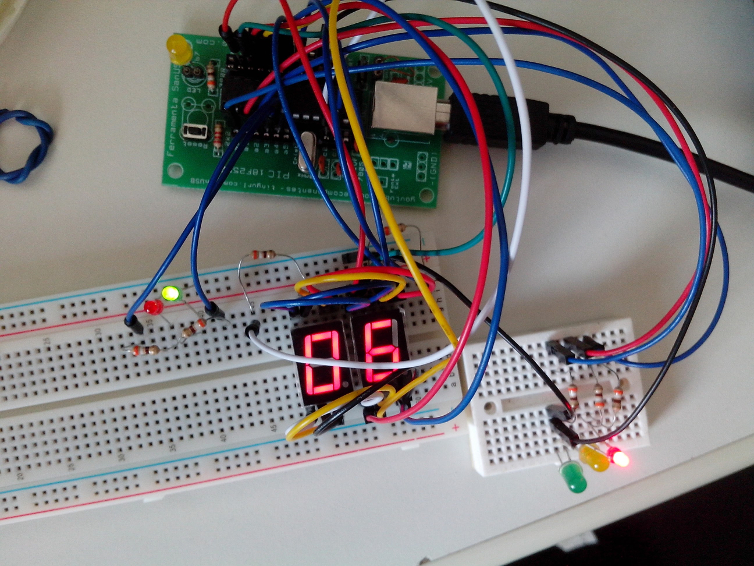
\includegraphics[scale=0.5]{img/IMG_20161208_100054.jpg}
    \caption{Circuito}\label{fig:montagem}
\end{figure}
